\documentclass{article}
\usepackage{graphicx} 
\usepackage{hyperref}
\hypersetup{
    colorlinks=true,
    allcolors=black
}
\usepackage{braket}
\usepackage{titlesec}
\usepackage{geometry}
\usepackage{minted}
\usepackage{amsmath}
\usepackage{xcolor}
\usepackage{comment}
\usepackage{quantikz}

\newcommand{\ec}{\gate[style={draw,minimum width=0.55cm,minimum height=0.45cm}]{\text{\scriptsize EC}}}
\newcommand{\leftlabel}[2]{\llap{\smash{#1}\quad}#2}

\geometry{a4paper, margin=1in}
\setlength{\parindent}{0pt}
\usepackage{subfig}

\usepackage[backend=bibtex, style=numeric, sorting=none]{biblatex}
\addbibresource{references.bib}

\title{Atom Loss Tolerant QEC on Neutral Atom Arrays}
\author{Adeniyi Osinowo}

\date{\today}

\begin{document}

\maketitle

\begin{abstract}
Neutral atom arrays have emerged as a leading platform for scalable fault-tolerant quantum computing, but their performance is strongly constrained by atom loss.
In this review, atom loss is treated as an architectural challenge for quantum error correction (QEC), particularly because loss events violate the standard fixed-qubit assumptions.
It is discussed how loss can be converted into flagged erasures, enabling erasure-aware decoding and improved thresholds relative to standard Pauli-noise models.
Recent hardware-efficient strategies are examined in which qubits are engineered so that dominant physical noise channels are made more correctable, and are then concatenated with codes matched to those noise characteristics.
A holistic perspective is adopted in which code structure, decoder design, and noise modelling are considered jointly for neutral-atom systems.
The review therefore focuses on pathways for integrating fast, reliable loss detection and recovery into scalable neutral-atom architectures while managing control overhead and implementation complexity.
\end{abstract}

\section{Introduction} 
Since their experimental realization in the early 2000s, neutral atom arrays were largely regarded as scalable but slow, low-fidelity platforms that were better suited to quantum simulation than to universal quantum computation. % Add references for early neutral atom arrays
In recent years, substantial progress has been achieved, including high-fidelity single-qubit gates~\cite{PhysRevLett.121.240501}, two-qubit entangling gates~\cite{Cesa_2017}, and large-scale arrays containing hundreds of atoms~\cite{bluvstein2024logical}.
As a result, neutral atom arrays have been established as strong candidates for scalable fault-tolerant quantum computing, with key advantages such as mid-circuit reconfigurability, long coherence times, and highly parallel entangling operations.
For fault tolerance to be realized on this platform, high-speed operation with high-quality qubits at large scale is required.
Under standard quantum error correction (QEC) approaches, however, the target error regimes are typically reached only with very large physical-qubit overheads \cite{Fowler2012SurfaceCodes, Riverlane2025QEC}.
One of the key challenges in achieving this is atom loss, which can compromise the effectiveness of QEC strategies on this platform. \\

In neutral atom arrays, individual Rydberg atoms are trapped in optical tweezers, quantum gates are implemented with laser pulses, and readout is performed by fluorescence imaging.
During these operations, atom loss is induced by collisions, spontaneous emission, and trapping imperfections \cite{bluvstein2024logical}.
In contrast to standard bit-flip and phase-flip errors, atom-loss events are often heralded: the error location is known, but the qubit state is destroyed.
Consequently, conventional QEC assumptions of a fixed qubit set with hidden errors inferred only through syndrome data are violated.
Although undetected loss can produce logical failure, detected loss can be converted into flagged erasures, and improved decoding performance and higher physical error thresholds have been reported relative to standard Pauli-noise settings \cite{gu2024optimizing, chang2024surface, gu2023fault}.
The central challenge is implementing fast, reliable loss detection with low false-positive rates and overhead.

To address this challenge, hardware design now focuses on explicitly engineering qubits so their dominant noise source can be corrected more efficiently \cite{wu2022erasure, kubica2023erasure, teoh2023dual, scholl2023erasure, kang2023quantum, koottandavida2024erasure, gu2023fault, levine2024demonstrating, hann2024hybrid, guillaud2021error, guillaud2019repetition, xu2023autonomous}.
This approach achieves significantly better error thresholds and reduces the physical-qubit overhead required for fault tolerance as hardware-efficient QEC can be tailored to the dominant noise channel, and decoders can leverage the additional information provided by heralded loss events.
The main remaining bottleneck is scale: achieving useful logical error rates still requires large physical-qubit counts and substantial control overhead. 
A central design objective is therefore to integrate fast, reliable loss-detection and recovery directly into hardware while keeping added complexity and scaling costs manageable.
This review focuses on atom-loss-tolerant QEC for neutral-atom arrays with a holistic approach considering the interplay between the code, decoder, and noise model in achieving fault tolerance. 
To begin the exploration of hardware-efficient QEC tolerant to atom loss, this review will cover the background of qec and neutral-atom hardware.

    \subsection{QEC background} \label{subsec:qec-background} % Add mathematical definitions and notation for QEC
    % - Paragraph: Introduce in detail QEC and the threshold theorem framework of QEC & Explain that this study will focus on exploring each aspect
    QEC refers to techniques that suppress the effective error rate of quantum computations by encoding one logical qubit into many physical qubits, then repeatedly detecting and correcting faults without directly measuring the logical state.
    Error correction alone is not sufficient for scalable quantum computing. 
    Fault tolerance as described by threshold theorem requires a more holistic approach that also takes in to account the quality of the Error Model, Code, and Decoder and there exists a physical error rate below which increasing code distance suppresses logical error \cite{aharonov1997fault, knill1998resilient, kitaev2003fault}.
    Operating below threshold is therefore the key practical criterion, and has become a central benchmark in recent experiments \cite{google2024quantum}.
    At a high level, the QEC cycle has three components: encoding, error detection, and decoding \cite{NielsenChuang, Gottesman1997, PreskillNotes}. \\

    \textbf{Types of Errors}\\
    % - Paragraph: Introduce the types of quantum computing errors & compare quantum vs. classical errors & explain the concept of erasure errors & Establish heirarchy of errors: compare erasure(correctable) vs. Pauli(detectable) and leakage errors(undetectable).
    Qubits are generally susceptible to a wide variety of error types, which can be broadly categorized into three classes: leakage errors, Pauli errors, and erasure errors.
    Leakage errors are the most harmful because they take the qubit out of the computational subspace, and are undetectable without additional hardware.
    Pauli errors stay within the computational subspace and can be detected and corrected by the error-correcting code.
    Erasure errors are initially undetectable but can be flagged by erasure checks, allowing for efficient correction. \\

    \begin{figure}[h!]
        \centering
        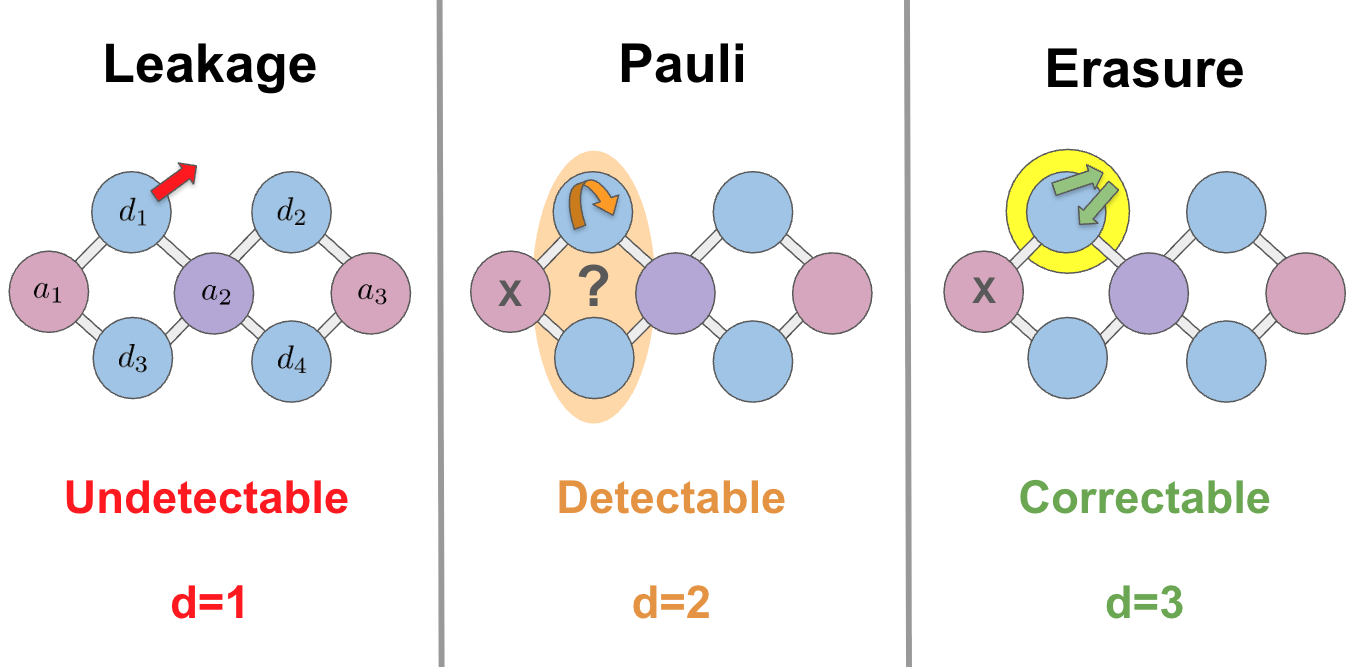
\includegraphics[width=0.8\linewidth]{errorhierarchy.png}
        \caption{Comparison of leakage, Pauli, and erasure errors in a minimal surface-code layout, with data qubits $d_i$, ancilla qubits $a_i$, and effective code distance d. Leakage errors escape the computational subspace without any flag (undetectable, distance $d=1$);  
        Pauli errors stay within the subspace and flip stabilisers (detectable, $d=2$);  
        erasure errors initially escape the computational subspace, then are flagged by erasure checks and can be reset and corrected (correctable, $d=3$).}
        \label{fig:error-types}
    \end{figure}

    These error types form a hierarchy of increasing detectability and correctability, with leakage errors being the most harmful and erasure errors being the most benign.
    Hardware-efficient QEC strategies therefore aim to engineer qubits so that the dominant noise channel is erasure errors, which can be efficiently detected and corrected, while suppressing leakage and Pauli errors as much as possible.\\

    \textbf{Encoding}\\
    % - Paragraph: Families of codes, and their properties (surface code, qLDPC codes, etc), outline factors to consider when choosing a code (overhead, connectivity, decoding complexity)
    Encoding maps logical states into an entangled code space so that local physical errors can be detected and corrected while preserving the encoded information.
    Different code families make different trade-offs between overhead, connectivity, and decoding complexity. 
    Surface codes are currently the most mature for local 2D hardware because they rely on nearest-neighbour stabiliser checks and have high practical thresholds, but they require substantial physical-qubit overhead. 
    High-rate qLDPC codes can encode more logical qubits per physical qubit, potentially reducing overhead, but typically demand more complex check graphs and fault-tolerant implementations.\\

    % - Paragraph: How QEC codes detect errors (stabilizer formalism and syndrome extraction, Difficulties of error detection), outline factors to consider when designing error detection (frequency of checks, placement of checks, etc)
    % Unlike classical codes, QEC cannot identify errors by directly reading out data qubits, because direct measurement collapses superpositions and destroys the encoded state.
    % The key idea is to measure commuting stabiliser operators, usually through ancilla qubits, so that only error information is extracted. These measurements produce a classical \textit{syndrome}: a pattern of violated checks indicating where and what type of faults are likely to have occurred \cite{calderbank1996good, steane1996multiple}.
    % Syndrome extraction is repeated over many rounds to separate true data errors from noisy measurements. In practice this step is difficult because ancilla preparation, entangling gates, and readout are themselves imperfect, so the detection circuit must be fault-tolerant.\\
    % In recent years, there has been increasing interest in \textit{high-rate qLDPC codes} which can have a higher encoding rate of logical qubits per physical qubit than the surface code \cite{breuckmann2021quantum}. 
    % For example, IBM Quantum published research into the bivariate bicycle code \cite{bravyi2024high, yoder2025tour}. 
    % These codes have potentially large savings in qubit count, though for superconductors there is a hardware challenge of implementing long-range gates. 
    % While these codes typically require significant hardware modifications for superconductors, a recent proposal from Riverlane researchers identifies a new family of high-rate qLDPC codes known as \textit{directional codes}, which can be implemented on local connectivity \cite{geher2025directional}. 
    % Unlike the surface code, there are not standard methods for implementing fault-tolerant logical operators with qLDPC codes, though IBM researchers recently published progress in this direction \cite{yoder2025tour}. 
    % The 2024 and 2025 Riverlane QEC reports therefore summarised qLDPC codes as a ``high risk, high reward" approach to quantum error correction \cite{riverlane2024quantum, Riverlane2025QEC}. \\
    \begin{figure}[h!]
        \centering
        \begin{quantikz}[row sep=0.35cm, column sep=0.45cm]
            \lstick{$d_1$} & \qw & \ctrl{4} & \ec & \qw & \ec & \qw & \ec & \qw & \ec & \qw \\
            \lstick{$d_2$} & \qw & \qw & \ec & \ctrl{3} & \ec & \qw & \ec & \qw & \ec & \qw \\
            \lstick{$d_3$} & \qw & \qw & \ec & \qw & \ec & \ctrl{2} & \ec & \qw & \ec & \qw \\
            \lstick{$d_4$} & \qw & \qw & \ec & \qw & \ec & \qw & \ec & \ctrl{1} & \ec & \qw \\
            \leftlabel{$a_Z$}{\ket{0}} & \qw & \targ{} & \ec & \targ{} & \ec & \targ{} & \ec & \targ{} & \ec & \meter{}
        \end{quantikz}
        \caption{Syndrome extraction circuit for a $d=2$ surface code with integrated erasure checks.  
        The data qubits $d_i$ and ancilla $a_Z$ are dual-rail encoded qubits.  
        Each erasure check flags leakage out of the computational subspace, after which the affected qubit is reset before continuing the circuit.}
        \label{fig:erasure-circuit}
    \end{figure}
    % Use the factors introduced in {QEC Background} to rank the codes
%     Erasure checks are performed after each gate. 
%     If a check flags, the corresponding qubit is reset to the computational subspace $\{\ket{01},\ket{10}\}$, a process known as \textit{erasure conversion}. 
%     For analysis and simulation, this reset is often treated as producing a maximally mixed state in that subspace, so the resulting error channel is equivalent to a depolarising (Pauli) channel. 
%     The stabiliser measurement on $a_Z$ then identifies the error type, while the erasure flag identifies the location. 
%     Together, these two pieces of information make the error fully correctable. \\ 

%     There are many other codes with their own benefits and drawbacks that are attracting significant research interest, including color codes \cite{Bombin2006ColorCodes,Landahl2011ColorCodes} and Floquet codes \cite{Hastings2021Floquet,Fahimniya2025HyperbolicFloquet}.\\

%     The $n=4$ surface code example also clearly illustrates the hierarchy of erasure, Pauli and leakage errors, which each have a different effective distance and resulting protection against errors, depicted in figure~\ref{fig:error-types}. \\

%     In addition to the four data qubits, $d_1$–$d_4$, the figure shows three ancilla qubits; two to check for X-errors on the computational states of these data qubits (bit-flips) and one to check for Z-errors (phase-flips). 
%     Specifically, in this example ancilla $a_1$ checks for $X$-errors on $d_1$ or $d_3$; $a_2$ checks for $Z$-errors on $d_1$, $d_2$, $d_3$, or $d_4$; and $a_3$ checks for $X$-errors on $d_2$ and $d_4$.  
%     The ancillas begin in the state $\ket{000}$, and their measurements yield a three-bit syndrome pattern that reveals which stabilisers were violated.  \\

%     For a single Pauli error, the ancillas that change state indicate whether the error was of $Z$-type (via $a_1$ or $a_3$, syndromes 100 or 001), $X$-type (via $a_2$, syndrome 010), or $Y$-type (via both $a_2$ and either $a_1$ or $a_3$, syndromes 110 or 011). 
%     Hence, for arbitrary Pauli noise, a single error can always be detected; however, there is ambiguity about which data qubit produced that syndrome, since multiple error locations share the same stabiliser check outcomes.\\

%     When the underlying noise is instead erasure noise, each erasure check directly identifies the data qubit $d_i$ that left the computational subspace.  
%     The syndrome then provides the error type while the erasure flag gives the location, resolving this ambiguity and enabling full correction of the error. \\ 
% Code distance is defined as the minimum weight error that will not be detected by the code, with \textit{weight} being the number of qubits that are affected by the error. 
% In \cite{grassl1997codes}, it was shown that a code of distance $d$ can correct any $d-1$ or fewer erasure errors, compared with the standard limit of $\left\lfloor \frac{d-1}{2} \right\rfloor$ arbitrary errors. 
% The former follows directly from the fact that $d-1$ errors can be detected in a distance $d$ code, with correction being possible with supplementary location information. 
% Hence there is a significant gain in the number of errors that can be corrected for a given code when including information about the location of errors. 
% An illustrative example is that while the smallest size code for correcting arbitrary errors requires five qubits, adding the location information of erasure errors reduces the minimum qubit number to four \cite{grassl1997codes} (see figure~\ref{fig:erasure-circuit} for an example of this result with the surface code). 
% This demonstrates how an erasure noise model enables a given number of physical qubits to have enhanced error-correction capabilities.\\

    \textbf{Decoding}\\
    % - Paragraph: How Decoding works: types of decoders, difficulties of decoding, outline factors to consider when designing decoders (accuracy, runtime, implementation cost)
    Decoding is the classical inference step that maps syndrome data to a likely error pattern and a corresponding recovery operation.
    For topological codes, widely used decoder families include minimum-weight perfect matching and Union-Find methods, which differ in accuracy, runtime, and implementation cost.
    The core challenge is degeneracy: many different physical error configurations can produce the same syndrome. Effective decoders therefore combine syndrome history with a realistic noise model and any side information (for example, heralded erasure locations) to minimise logical failure probability.\\

    \subsection{QEC on Neutral atoms} % Describe Threshold theorem framework for QEC on neutral atom arrays, and explain how this study will focus on exploring each aspect
    % - Paragraph: Describe neutral atom arrays architecture and physics behind its operation, and highlight how its advantages arise from its design & Discuss the performance and limitations of state of the art neutral atom arrays
    Neutral-atom quantum processors trap individually addressable atoms in optical tweezers or optical lattices and encode qubits in long-lived internal states. 
    Large, defect-reduced 2D/3D registers are built by loading and rearranging atoms with movable tweezers, and entangling gates are implemented by transiently exciting selected atoms to Rydberg levels ($n > 10$), where strong dipole-dipole interactions enable fast conditional dynamics. 
    The main advantages follow directly from this architecture: natural atomic uniformity minimizes device-to-device variability, optical trapping supports high-density scaling and reconfigurable connectivity via qubit shuttling, long-lived encodings provide extended coherence, and laser-based control in vacuum can support mid-circuit measurement/reset without requiring the heavy cryogenic infrastructure typical of superconducting platforms.\\

    \subsubsection{Neutral atom error profile} \label{subsec:neutral-atom-error-profile}
    % - Paragraph: Describe the error profile of neutral atom arrays & Explain focus on hardware-efficient QEC, and how it can be used to design hardware that takes advantage of the native noise profile of neutral atom arrays

%     In summary: leakage errors leave the computational subspace without any detectable flag, making them undetectable ($d=1$).  
%     Pauli errors stay within the subspace and flip stabilisers, making them detectable but not localisable ($d=2$).  
%     Erasure errors are both detectable and localisable. When an erasure check flags, the qubit’s location is known, and after erasure conversion the resulting Pauli-type error can be diagnosed and corrected by the stabilisers.  
%     The effective distance for erasure errors is therefore $d=3$, such that they are correctable.  

% Key detection techniques and methods of detecting atom loss:

%     Fluorescence Imaging: Atoms are trapped in optical tweezers, and when illuminated, they scatter photons (fluoresce). The absence of photons at a specific tweezer location indicates an atom has been lost.
%     Non-destructive Readout: Using a high-numerical-aperture microscope objective, atoms can be imaged in a cavity-enhanced 3D lattice, allowing for detection with high fidelity (over 99%) without significantly disturbing adjacent atoms.
%     Leakage Detection Units (LDUs): To avoid destroying the entire state of the quantum processor, small circuits (LDUs) can be attached to qubits to detect if an atom has escaped ("leaked" from) the trap.
%     Two-Image Sequence: To differentiate between a "0" state atom and a missing atom, a second image can be taken after an optical pumping pulse transfers all atoms to a bright state.
%     Repetition Code and Midcircuit Measurement: Researchers use repeated syndrome extraction to detect and correct atom loss in real-time, even replacing lost atoms with new ones from a reservoir

%     Other efforts to engineer noise of superconducting qubits include bosonic encodings such as cat qubits, which realize strongly biased Pauli noise. 
%     At suitable operating points, bit-flip processes are exponentially suppressed relative to phase-flip processes \cite{mirrahimi2014dynamically, tuckett2018ultrahigh, roffe2023bias}. 
%     This biased Pauli noise can be leveraged by tailored decoders and codes, so the code concentrates on the dominant error channel, increasing threshold and encoding rate. 
%     The approach is being actively explored by academic groups (e.g. Yale, Caltech) and industry (e.g. Alice $\&$ Bob, AWS), with small-scale demonstrations exhibiting the requisite biased noise \cite{reglade2024quantum, hann2024hybrid, putterman2025hardware}. 
%     Theoretical thresholds and physical qubit resource savings under Pauli biased noise have been analyzed for several code families \cite{mirrahimi2014dynamically, tuckett2018ultrahigh, roffe2023bias}. 
%     Another bosonic approach is the GKP (Gottesman-Kitaev-Preskill) code, which converts continuous displacement noise into X- and Z-type error syndromes. 
%     Employed as an inner code, GKP can substantially lower qubit-number overhead via concatenation with outer codes such as the surface or XZZX code \cite{Conrad2022GKPcodes, Zhang2023ConcatenationGKPXZZX}. \\

%     The flexibility of hardware errors to deviate from standard Pauli noise models is therefore not only a challenge, but an opportunity: quantum error-correcting codes can be adapted to take advantage of the unique features of hardware noise, and qubits can be intentionally designed to exhibit errors that can be corrected more efficiently. 

    \subsubsection{Encoding on neutral atoms}
    % Discuss implementations of QEC codes on neutral atom arrays(explain the physical processes involved)
    To see how an erasure error-correction protocol operates in practice, consider the surface-code syndrome extraction circuit in figure~\ref{fig:erasure-circuit}.  
    The four data qubits $d_i$ form a surface code, and the ancilla $a_Z$ measures a $Z$-type stabiliser that flags $Z$ errors on the data qubits.  
    Both data and ancilla are dual-rail encoded qubits, so erasure checks can be applied throughout the circuit.  \\

\section{Atom loss error model}
% - Paragraph: Methods of representing errors
% This section will explain how erasure qubits can be implemented using dual-rail encoding, and review analytic and numerical results on how they increase the power of quantum error-correcting codes. 
% Two standard modelling levels are widely used: the \textit{circuit noise} model and the \textit{phenomenological noise} model \cite{dennis2002topological, fowler2009high, wang2011surface}.
% Circuit-level models inject faults at each operation in the full syndrome-extraction circuit (state preparation, gates, idling, and readout), whereas phenomenological models apply effective errors directly to data qubits and measurement outcomes at fixed rates.
% Although less realistic, the phenomenological model is computationally efficient and useful for scaling studies. 
% More general hardware noise is often reduced to effective Pauli channels via Pauli twirling~\cite{twirling}, enabling stabiliser-based simulation and decoder benchmarking.\\

% The dominant errors on erasure qubits cause a qubit's state to leave the standard computational subspace, followed by a measurement that detects this error. 
% When an error that leaves the computational subspace is detected, it is termed a \textit{heralded erasure} or \textit{erasure error}. 
% By contrast, an error that leaves the computational subspace and is not detected is leakage, a harmful source of noise introduced in section \ref{subsec:qec-background}. 
% Erasure errors are leakage errors that are engineered to be detectable, enabling powerful error-correction properties. 

% % - Paragraph: Recent advances in erasure QEC theory and simulation
% Erasure noise has been demonstrated in circuit-level noise simulations and theoretical analysis to enable increased threshold and reduced logical error probability in the surface code, with one study analysing frequency of erasure checks finding an approximately 50$\%$ increase in threshold  \cite{gu2024optimizing} and another focused on imperfect erasure checks finding threshold at least over twice that of Pauli noise \cite{chang2024surface}. 
% Gains in threshold and sub-threshold scaling have also been found for Floquet codes \cite{gu2023fault}. \\

% In the case of high-rate quantum LDPC codes, a study of the La-cross code and bivariate bicycle code found orders of magnitude reductions in logical error probability \cite{pecorari2025quantum}. 
% The threshold improvement of the La-cross code with erasures was similar to the surface code, though the bivariate bicycle code did not show significant threshold improvements. 
% Numerical results therefore suggest that the magnitude of increase in threshold depends on the details of the code, while significant improvements to sub-threshold scaling and logical error probability apply for arbitrary codes.  
% In general, it is expected that erasure qubits will benefit any code they are concatenated with, though finding which codes benefit most from erasure qubits and characterising impacts on threshold and logical errors is an active area of research \cite{gu2023fault}.\\

% Recent work showed that incorporating erasure-location information can dramatically raise the fault-tolerance threshold of a code . 
% In the idealised limit of perfect syndrome measurements (the \textit{code-capacity} noise model), the surface-code threshold with location information reaches $50\%$, whereas without location information the corresponding depolarising-noise threshold is upper-bounded at around $19\%$ \cite{Wootton2012HighThreshold, Bombin2012StrongResilience}. 
% This $50\%$ value saturates the fundamental bound imposed by the no-cloning theorem.\\ 

% A further advantage comes from \textit{biased} erasure noise, where not only the location of the error but also the specific state involved in the decay is known. 
% This scenario arises naturally in architectures where only one of the dual-rail basis states undergoes amplitude damping. 
% The resulting erased qubit can then be reset back to the computational state from which it decayed, creating a bias in the effective Pauli errors in the qubits, which can be exploited by the decoder \cite{sahay2023high}. 
% Recent theoretical studies \cite{sahay2023high, wu2022erasure} show the significant improved performance that such biased erasures can achieve relative to symmetric erasures. In particular, thresholds can increase by factors of approximately 2–5, depending on the bias ratio and code family, and logical error rates at fixed physical error can be correspondingly reduced.\\

% A recent study additionally found significant benefits to using erasure qubits for implementing non-Clifford gates, with both analytical results and numerical simulations \cite{jacoby2025magic}. 
% They considered magic-state distillation using the surface code. 
% A distillation protocol requires first using magic-state injection circuits to prepare low-error magic states, that are then used for distillation to lower-error states. 
% The injection process involves error-detection, and postselection on the states without errors. In simulations of magic-state injection protocols with erasure qubits, they were found to have significantly lower logical error rates than with the standard Pauli noise. 
% Meanwhile, the acceptance rate was only marginally reduced. Similarly, logical error rate savings were also found for the cultivation step of the magic-state cultivation protocol, which was recently proposed to prepare high-fidelity magic states at substantially lower overhead than traditional distillation \cite{gidney2024magic}.\\

% Based on this, the authors of \cite{jacoby2025magic} estimated that erasure qubits used together with magic state cultivation can achieve the error-rate required for early fault-tolerant quantum applications with physical (heralded) erasure error rates less than around $4 \times 10^{-3}$, and residual Pauli error rates of order $10^{-4}$. 
% This demonstrates an important tipping point for superconducting qubits: the physical error-rates required for low logical error rates are becoming realistically achievable using near-term hardware.\\

% - Paragraph: Discuss and assess existing error models to identify which are the most accurate for atom loss.

\section{Atom loss QEC codes} 
% - Paragraph: Describe implementations and results/performance(scalability and detection performance) of loss-aware codes strategies
Existing qubit loss–aware code strategies for neutral-atom arrays now span four main approaches: 
(i) surface codes augmented with dedicated loss detection and loss-aware decoding, 
(ii) architectural schemes that relocate logical qubits away from accumulated erasures, 
(iii) fully experimental surface-code implementations that exploit loss information via “superchecks” and machine-learning decoders, and 
(iv) dual-rail encodings that natively map qubits onto an erasure model. 
Together, these works show that treating atom loss as an erasure with known location can significantly raise effective thresholds and improve logical performance, with dual-rail encodings providing a particularly clean mapping from physical loss processes to erasure errors at the code level. 
In neutral-atom platforms, dual-rail approaches can be realized either via two-atom encodings or via internal-level encodings that ensure loss or leakage produces a detectable vacancy, making them highly compatible with erasure-oriented decoders.\\

% - Paragraph: Discuss the performance of erasure error-correcting codes
Surface-code schemes with loss detection units (LDUs) exemplify the first class: LDUs identify lost atoms each cycle, feed explicit erasure locations to an adaptive decoder, and achieve orders-of-magnitude reductions in logical error probabilities relative to loss-agnostic decoding, with threshold lines that trade off tolerated loss versus depolarizing noise. 
These schemes scale naturally in code distance, require only local detection plus more sophisticated decoding, and become even more accurate when combined with dual-rail encodings or erasure-conversion techniques that convert leakage and other faults into flagged erasures, thereby aligning the physical noise more closely with the assumed erasure model.\\

Erasure-recovery architectures such as k-shift protocols address long-time operation in dense arrays, where erasures accumulate and naive refilling leads to vanishing effective thresholds. 
They periodically deform the surface code and transport atoms so that the logical patch is shifted away from damaged regions into freshly prepared ones, restoring practical logical error suppression at finite distances that are realistic for near-term devices but at the cost of code-deformation overhead and large-scale rearrangement.
Dual-rail encodings can be integrated here by moving logical dual-rail pairs rather than single sites, using one rail as a sacrificial channel for loss, which stabilizes the effective erasure pattern seen by the decoder while increasing physical-qubit overhead.\\

Large-scale neutral-atom experiments implement surface codes with explicit loss-aware decoding by forming “superchecks” (products of stabilizers around lost atoms) and training most-likely-error or machine-learning decoders on loss patterns, thereby recovering syndrome information and reaching below-threshold logical performance in multi-round QEC experiments. 
These demonstrations validate that loss-aware strategies are experimentally viable at the few-hundred–atom scale and provide a natural setting for dual-rail encodings, where decoders can directly exploit structured correlations between rail occupations, loss events, and stabilizer outcomes \cite{perrin2024quantum}.\\

% - Paragraph: Discuss the performance of erasure error-correcting codes
Overall, LDUs and superchecks with loss-aware decoding appear most accurate and scalable as code-level treatments of atom loss, while dual-rail encodings and erasure-conversion schemes are most effective at cleaning up the physical noise so that it matches an erasure model. 
Erasure-recovery via k-shift–type protocols becomes important when loss is strong and densely packed arrays limit local refilling, and it can be combined with dual-rail encoding to make the motion of logical information more robust. 
The emerging consensus is that the most accurate, scalable neutral-atom architecture for atom loss will combine dual-rail or erasure-converted qubits, real-time loss detection (LDU-like mechanisms), superchecks plus loss-aware decoding, and periodic patch relocation when erasure density becomes too high.\\

\section{Atom loss Decoding}
Loss-aware decoding strategies have emerged as a crucial ingredient for achieving fault tolerance in architectures where qubit loss or erasure is a dominant error channel, including neutral-atom arrays. 
These approaches exploit additional information provided either by active loss detection units (LDUs), by encoding (dual‑rail), or by code‑deformation tools such as superchecks and k‑shift protocols, to convert loss into a structured erasure pattern that can be handled more efficiently than generic Pauli noise. 
At a high level, all of these strategies trade hardware or control overhead for a substantial reduction in logical error rates at realistic loss probabilities, but they differ in how aggressively they use loss information and in how forgiving they are to imperfect detection.\\

Strategies based on loss detection units integrate additional measurements into the surface-code cycle to flag lost atoms before or during stabilizer extraction. 
In the atom-loss–resilient surface-code construction for neutral atoms, standard LDUs and teleportation‑based LDUs are compared via circuit‑level simulations under combined atom loss and depolarizing noise. 
Both variants feed explicit loss locations into a loss‑aware decoder, which effectively works on an erasure channel overlaying a Pauli channel. 
Simulations show that including LDUs can improve logical error probabilities by orders of magnitude at fixed physical error rates, and that an atom‑loss threshold on the order of a few percent is achievable when depolarizing noise is sufficiently low. 
Teleportation‑based LDUs tend to be more robust to detection-induced back‑action but require additional ancillae and gates, whereas standard LDUs are simpler but somewhat more sensitive to measurement errors.\\

Dual‑rail encoding takes a different route by embedding loss detection directly in the logical qubit definition. 
In cavity and superconducting implementations, the logical states are encoded in single‑excitation subspaces of two modes, so that dominant photon‑loss events manifest as erasures that can be detected via syndrome‑like checks or post‑selection. 
In dual‑rail cavity qubits, error‑detection protocols convert most physical amplitude damping into flagged erasures, leaving a background of Pauli‑like errors that is orders of magnitude smaller than the original noise. 
Experiments with dual‑rail encoded multimode transmons demonstrate logical bit‑flip and phase‑flip error rates more than an order of magnitude lower than the physical ones, with stability over hours‑long runs; this confirms that hardware‑level erasure detection can deliver a highly favorable hierarchy of error rates for downstream QEC decoders. 
While these works do not implement large‑distance codes, they indicate that when loss is the dominant channel, dual‑rail encoding can supply exceptionally clean erasure information to any standard erasure‑aware decoder.\\

In neutral‑atom surface‑code experiments, superchecks and related loss‑aware decoding schemes have been used to compensate for atom loss during stabilizer measurements. 
A recent fault‑tolerant neutral‑atom architecture demonstrates the use of superchecks, constructed by multiplying stabilizers surrounding a lost atom, to recover parity information that would otherwise be missing.
The loss pattern is then incorporated into both maximum‑likelihood and machine‑learning decoders trained on simulated and experimental data.
The authors compare different strategies-treating loss as $\ket{0}\ket{0}$, explicit loss detection without superchecks, supercheck construction, and post-selection on fully populated detectors—and show that superchecks combined with loss-aware decoding significantly suppress the detected error probability relative to loss‑ignorant schemes.
This confirms earlier theoretical predictions that exploiting erasure information in the decoder can strongly enhance surface-code performance in the presence of atom loss.\\

The k‑shift erasure‑recovery protocol for neutral‑atom surface codes pushes loss awareness further by combining code deformation with physical rearrangement of atoms. 
In this scheme, erasures (lost atoms) are corrected not simply by local superchecks, but by repeatedly transferring the logical qubit from an imperfect array with accumulated erasures to a pristine one, while correcting erasures in the emptied region using tweezers and atom transport. 
The decoder operates on dynamically deformed codes where stabilizers are redefined to avoid erased sites; numerical simulations show that k-shift erasure recovery restores the threshold behavior of the surface code in regimes where accumulated erasures would otherwise destroy its error‑correcting capability. 
Compared with simply repeating syndrome measurements on a static array, incorporating k-shift yields a substantially reduced logical failure rate at fixed physical loss and depolarizing rates.\\

Comparing these approaches, the most effective strategies are those that (i) achieve high-fidelity, near-real-time identification of loss events, and (ii) feed this information into a decoder explicitly designed for erasures rather than generic Pauli noise. 
LDUs on neutral‑atom surface codes achieve this with relatively modest overhead and already reach atom-loss thresholds of a few percent, especially when combined with teleportation-based detection that limits back-action. 
Superchecks are particularly powerful in experimental settings because they allow standard decoders (maximum-likelihood or machine-learning based) to operate on effectively complete syndrome information even in the presence of loss, leading to clear reductions in detected error rates. 
The k‑shift protocol appears most advantageous at higher steady‑state loss rates, where static-patch strategies fail, but its performance gains come with significant control complexity due to repeated code deformations and atom transport. 
Dual‑rail encoding provides arguably the clearest erasure channel and the lowest logical error per physical loss event, but it shifts the overhead into hardware resources (extra modes or qubits per logical qubit) and thus is most natural for platforms where bosonic or multimode structures are readily available. 
Overall, for qubit‑loss–aware codes in neutral‑atom arrays, hybrid schemes that combine local LDUs and superchecks with erasure-tailored decoders look most practical near-term, while k-shift protocols offer a promising route to maintain fault tolerance in regimes of sustained, high atom loss.\\

\section{Conclusion}
% Summarise the key points of the section, and discuss the implications for the field of quantum computing, and future directions for research in this area.
% The bottleneck for achieving useful quantum computing with superconducting qubits is the short T$_1$ times, caused by amplitude damping errors \cite{kubica2023erasure}. 
% Importantly, the physical error rate must be below threshold for quantum error correction in order to enable large-scale fault-tolerant quantum computing. 
% Recent developments with dual-rail superconducting erasure qubits give a promising solution: by engineering the noise of superconducting qubits to be detectable erasures, the dominant source of error in superconducting qubits can be efficiently corrected. 
% The threshold error can be significantly increased, up to realistically achievable rates with current and near-term qubits. 
% In addition, logical error with detectable erasures is reduced, meaning a lower ratio of physical qubits to logical qubits is required for achieving a given code distance. \\

% Recent simulations and proof-of-principle demonstrations show that these theoretical advantages carry over to realistic hardware. 
% The erasure-qubit approach to QEC is now being explored across superconducting, neutral-atom and trapped-ion systems, each leveraging the dual-rail encodings that originate in photonic devices.\\

% The combination of theoretical advances and the maturity of today's superconducting qubits has fuelled the rapid transition from theory to simulation to demonstration of these techniques. 
% The close relationships of companies and academic research groups have also enabled new ideas from academic labs to be adopted and developed in industry settings with fast turnaround times. 
% However, even with this momentum, the implementation of erasure qubits remains in its infancy, with many open questions left to explore in order to characterise its full potential and take advantage of the various new degrees of freedom introduced by this approach.\\

% These early results are already shaping how the field thinks about scalable quantum computing architectures. 
% The quantum industry recognises that these devices require strategic co-design of hardware with quantum error correction, with features such as a large logical-to-physical qubit ratio; high thresholds to physical noise; and architectures whose complexity does not grow prohibitively as systems scale. 
% Engineering dual-rail superconducting erasure qubits provides an avenue to achieving these goals for early fault-tolerant devices. 
% It is also a demonstrative example of the innovation possible on future qubit designs, building on the principle of concatenating error-correcting properties of hardware with outer codes to directly address the dominant physical noise sources.\\

% Erasure qubits, and more generally hardware-efficient QEC, offers a credible route to lower-overhead, higher-performance logical qubits. 
% They therefore represent one of the most promising directions for advancing toward scalable, fault-tolerant quantum computing.

    \subsection{Open questions and avenues for progress}

    We have discussed several open questions which could lead to interesting further explorations in the near term. These include the possibility of modifying hardware designs to further optimise the advantage to be gained from engineering erasure noise, discussed in section \ref{subsec:neutral-atom-error-profile}, and the unknowns regarding which codes stand to gain most significantly from enabling erasure-based error correction.\\

    % \textbf{Optimisations}\\

    % There are also various other directions for optimisations that have begun to be explored in the literature. For example, one of these explored in \cite{gu2024optimizing} is the relevance of the protocol used for the reset of an erased qubit back to the computational subspace. This can for instance can be a \textit{unitary pulse} (which risks taking a good qubit outside the computational subspace in the case of a false-positive erasure check) or a \textit{one-way pulse} which sends any state to the computational subspace. Another degree of freedom explored in \cite{gu2024optimizing} is optimising the frequency of erasure checks, trading clock time (which increases risk of idle errors) for additional information about erasures.  A further area for investigation is having more detailed noise models to understand the effect of imperfections in the erasure checks, and the trade-offs involved, analysed in \cite{chang2024surface}. \\

    % There may also be optimisations possible regarding efficient decoding of the error patterns from erasure qubits. This will depend on the nature of the outer code, since the approach to decoding can differ vastly for different codes. Further developments of results based on detecting and mitigating leakage errors (e.g. \cite{ziad2024local}) may also have application to erasure error decoding, given that they also deal with errors produced by leaving the computational subspace that are detected and then reset.\\

    % \textbf{Software tools for erasures}\\

    % Erasure-based quantum error-correcting codes differ both structurally and practically from conventional codes that do not incorporate erasure information. These distinctions pose significant challenges for the direct application of existing design~\cite{crumble, loom} simulation~\cite{gidney2021stim, riverlane_qecx}, decoding~\cite{decoding} and resource estimation~\cite{azure_resource, bartiq, qualtran} tools, which are typically designed for depolarizing or Pauli noise models without erasure flags. As such, existing tooling need extensions and adaptations for erasure-based codes. Adaptation of existing tools and development of new ones focused on code concatenation and erasure codes is essential for accelerated development of the field.\\

    % In particular, tools that support flexible code concatenation schemes, hybrid error models, and erasure-aware decoding strategies are critical to unlocking the full potential of erasure codes. Leveraging information about the location of errors requires custom simulation pipelines, decoders, and performance metrics. The development of such specialized tooling will not only facilitate rigorous benchmarking of erasure codes but also accelerate their integration into practical fault-tolerant quantum computing architectures.\\
    % cudaq vs stim detector error model


\printbibliography

\end{document}
